\chapter{Metodología de la Investigación}
En este capítulo se presenta detalladamente la definición de los experimentos numéricos a desarrollar, de modo que puedan ser replicables por cualquier persona o grupo de estudio que desee hacerlo. 

Específicamente se muestra: 
\begin{itemize*}
	\item La filosofía bajo la cuál se llevaron a cabo los experimentos.
	\item La definición de las condiciones de borde, iniciales e información estática para el modelo.
	\item La configuración espacial y temporal de los 4 experimentos realizados y su justificación, presentando la información existente en la literatura.
	\item La configuración utilizada del proceso de asimilación de datos utilizado.
	\item Presentación de las métricas estadísticas a utilizar para la medición del error.
\end{itemize*}
\newpage
\section{Aspectos Generales}
\subsection{Filosofía de la Investigación}
El objetivo final esta investigación es poder obtener una buena predicción del potencial eólico para zonas complejas exigiendo al límite el modelo meteorológico de mesoescala WRF. 

A continuación se presentan algunos lineamientos generales acerca de la filosofía que se adopta para la metodología con el fin de lograr este objetivo y que tienen gran influencia en la manera en la que se configuraron ciertos aspectos numéricos de los experimentos o se tomaron ciertas decisiones en la programación, por lo tanto es importante explicitarlos.
\subsubsection{Lineamiento de Simulaciones Reales}
Se busca realizar las simulaciones de la manera mas real y operativa posible. O sea, antes de utilizar información idealizada o conveniente con respecto al resultado final, se prefiere utilizar datos medidos en terreno. La mayor influencia de esto recae en tres aspectos:
\begin{enumerate*}
	\item Las condiciones de borde laterales del modelo provienen de un modelo global altamente probado (GFS) y a las cuales se les realiza un análisis (asimilación de datos) con  gran cantidad de mediciones ubicadas a lo largo de todo el planeta.
	\item Las bases de datos para la orografía del suelo no se generan computacionalmente, sino que solo se utilizan aquellas que son el resultados de campañas de medición o información proveniente de satélites.
	\item Ídem a lo anterior, la información para el uso de suelo solo proviene de satélites, campañas de medición o investigaciones previas que entregan datos concluyentes para asignar, por ejemplo, el $z_0$ y la categoría de uso de suelo.
\end{enumerate*}
Esta metodología tiene como consecuencia que la calidad de los resultados obtenidos estará directamente relacionada con la calidad de la instrumentación usada para medir los datos de entrada. Esto contrasta con algunas simulaciones presentes en la bibliografía en donde muchas veces se utilizan condiciones de borde periódicas, suposiciones de atmósfera neutra, se fija un cierto perfil de velocidad, etc. En esta investigación se busca ser lo mas correcto con respecto a la tecnología existente y, por lo tanto, con la operatividad del sistema. Bajo este mismo criterio, se evita el ajuste de parámetros arbitrarios del modelo, siendo $c_k$ (clausura turbulenta) la única constante que se asigna.
\subsubsection{Lineamiento de Libertad de Información}
Siguiendo con la misma filosofía del software libre WRF, toda la investigación fue realizada utilizando solo código libre e información pública que se puede acceder a través de internet. El posproceso de los datos fue realizado en parte a través del lenguaje de gráficos \emph{NCL} y en parte en \emph{Python}, los scripts desarrollados para la automatización del proceso de asimilación de datos fue hecho en \emph{bash}. La información de las mediciones medidas en terreno para los dos casos a analizar se obtuvieron a través de la página web \url{http://rodeo.dtu.dk/}.
\subsection{Resumen de la Metodología}
Para esta tesis, se llevaron a cabo 4 simulaciones atmosféricas multiescala las cuales son separadas en dos casos de dos experimentos cada uno: uno en terreno plano (para validar la metodología) y otro en terreno complejo.

Las distintas etapas del proceso de experimentación se pueden listar como:
\begin{enumerate*}
	\item \textbf{Selección de Dominios: } Elección de los terrenos reales a simular y la configuración para el escalamiento dinámico, definiendo la cantidad de dominios a anidar.
	\item \textbf{Preproceso de Información:} Abarca la obtención e incorporación de las bases de datos de alta resolución al modelo, las condiciones de borde e iniciales y las mediciones reales para la asimilación.
	\item \textbf{Ejecución de Experimentos:} Se llevan a cabo las simulaciones en el siguiente orden: (i) Terreno plano sin DA (validación), (ii) Terreno plano con DA en un solo punto de control, (iii) Terreno complejo sin DA y (iv) Terreno Complejo con DA en múltiples puntos de control.
	\item \textbf{Posproceso:} Se obtienen los gráficos para las variables relevantes para el análisis en cada caso, se calculan las variables de segundo orden, se obtienen los espectros de energía cinética y se computan las métricas estadísticas.
\end{enumerate*}
\newpage
\section{Selección de Dominios}
\subsection{Caso I - Terreno Plano: Høvsøre}
 Debido a la naturaleza numérica-experimental de esta tesis, es necesario tener un caso de validación que permita aprobar la metodología a aplicar y si fuese necesario, calibrar ciertos parámetros. Como es estándar en predicción eólica, se utiliza un caso real lo mas cercano posible a terreno plano con estratificación térmica neutra, a modo de ser comparable con las teorías basadas en el flujo sobre terreno plano homogéneo. Las condiciones para este caso serán: (a) poseer análisis en la literatura y (b) que existan datos medidos de acceso libre, tal que se puedan a utilizar en la asimilación de datos. Un lugar que cumple con estas características es el terreno de Høvsøre.

 El terreno de Høvsøre corresponde a un área costera al oeste de Jutland en Dinamarca en donde se ubica la Estación Nacional de Pruebas para Turbinas Eólicas. Høvsøre es una granja agrícola plana, cuasi homogénea, con alteraciones en el flujo del viento debido a la presencia del Mar del Norte (1.7 [km] al oeste), el fiordo Nissum (950 [m] al sur), algunas casas, árboles y parches de cultivos (al este), la villa de Bøvlingbjerg (3 [km] al sureste) y 5 turbinas eólicas al norte de un mástil meteorológico situado al sur de la estación como se puede ver en la Figura \ref{fig:05_terreno_hovsore}.
 
 \begin{figure}[H]
 	\centering\frame{
 		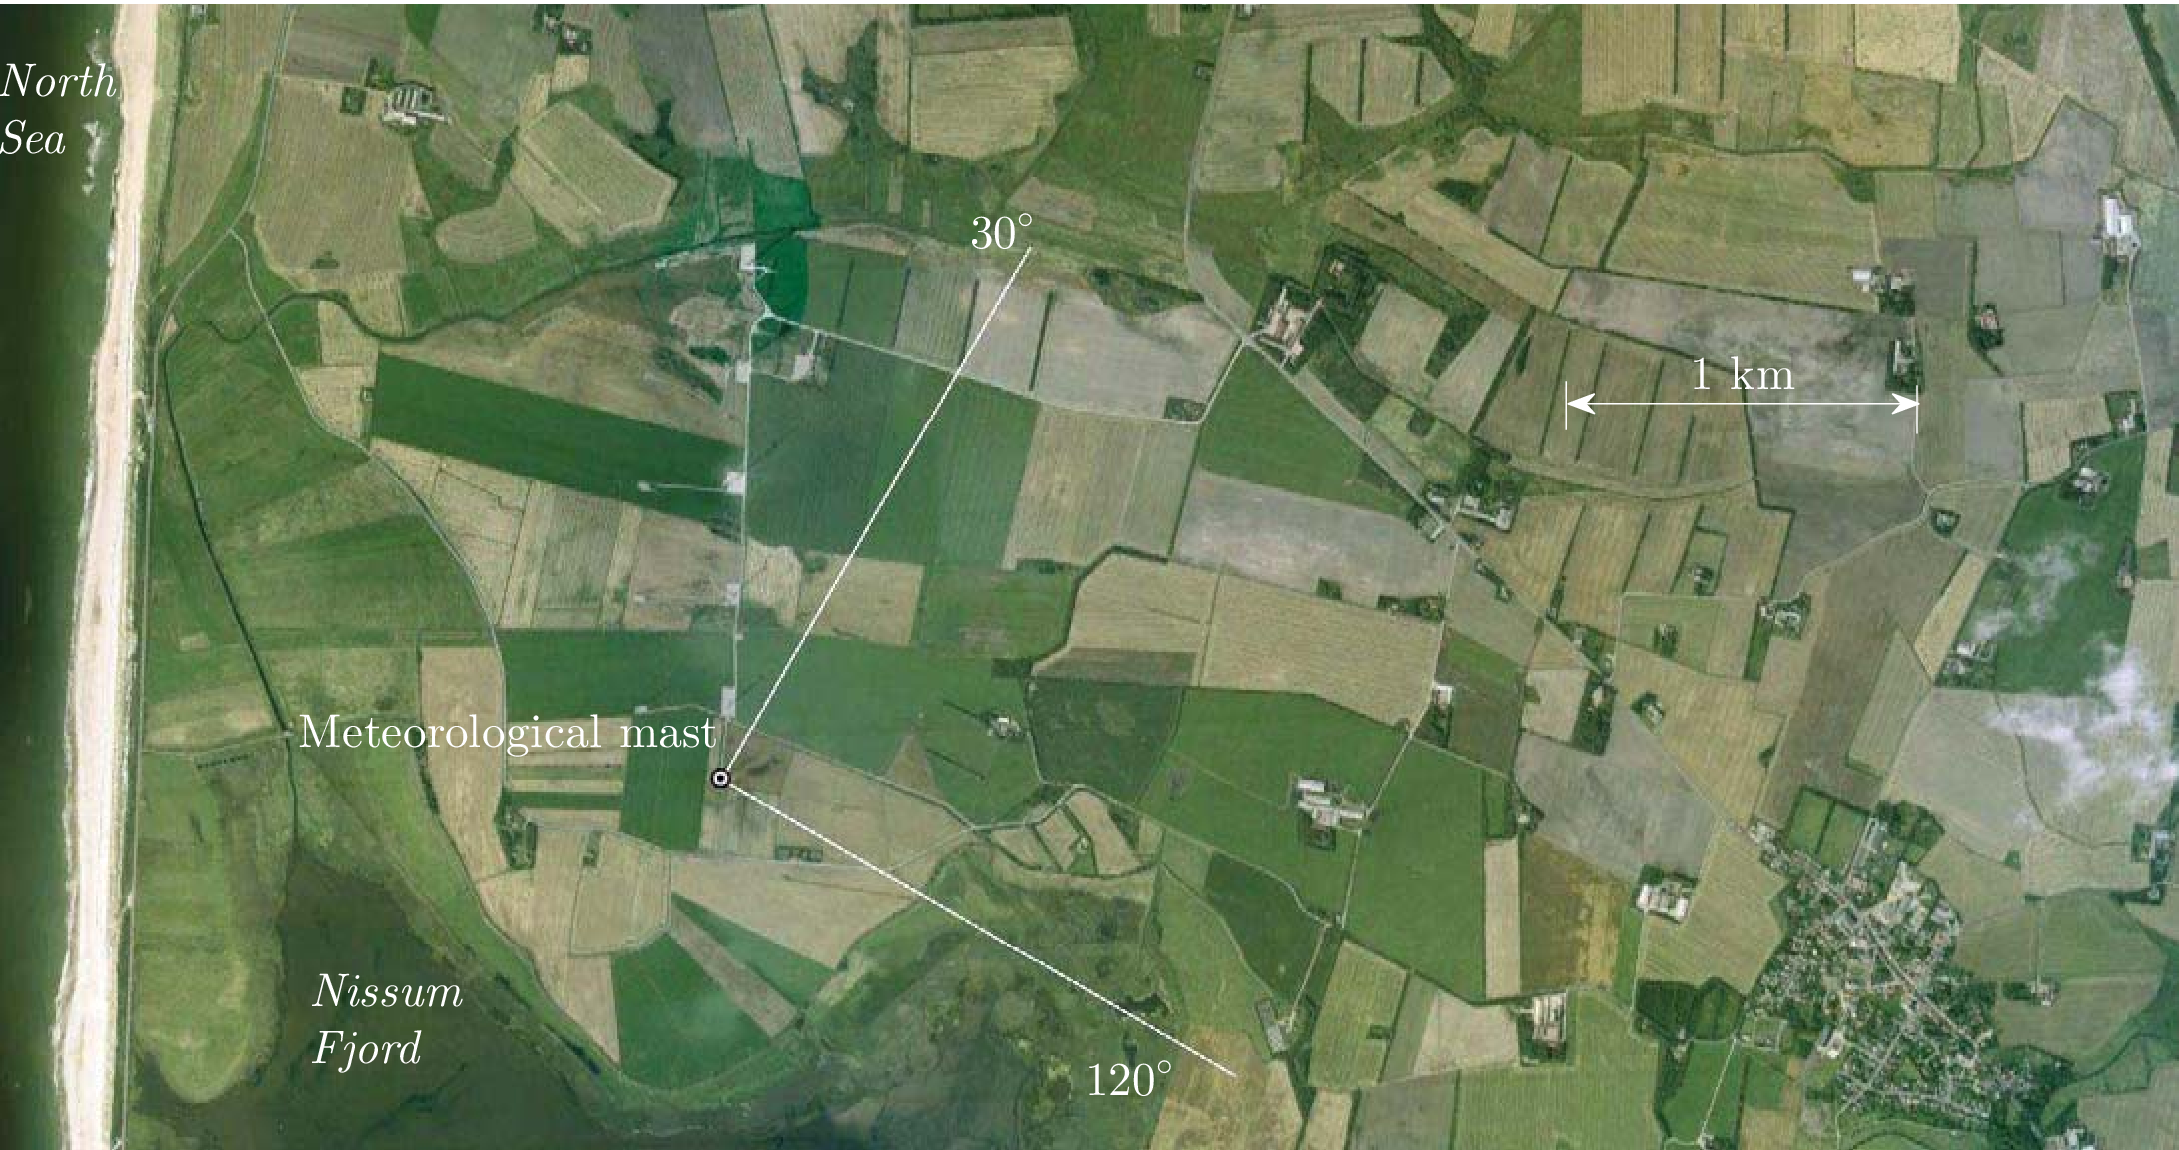
\includegraphics[width=0.98\linewidth,page=1,trim={0cm 0cm 0cm 0cm},clip]{Imagenes/05/hovsore}}%
 	\caption{Fotografía del terreno en Høvsøre. Fuente: \cite{Pea2013}}
 	\label{fig:05_terreno_hovsore}
 \end{figure}
 
 Los vientos provenientes del este (en el rango de los $30^\circ$--$120^\circ$), son entonces ideales para el estudio del viento sobre terreno plano y homogéneo, aunque estos generalmente no son típicos en este sitio.
 
 Para esta tesis, se utilizó el análisis y los resultados obtenidos por \cite{Pea2013}. En esa investigación se entrega un análisis de una base de datos de mediciones hechas en terreno a través de un anemómetro sónico y un lidar de viento junto con simulaciones mesoescala para todo el año 2010. El objetivo final es entregar un benchmark para viento sobre terreno plano (y por lo tanto es útil para este trabajo). Peña logra hacer una clasificación extensa del comportamiento del viento en Høvsøre y los separa en 10 casos según la dirección y la estratificación.
 
 El caso a comparar (para validar) será el caso 5, que corresponde a un viento de estratificación térmica neutra, atmósfera barotrópica y una dirección de viento superficial de $100^\circ$. Este caso está documentado para los días 07/09/2010 13:30-17:00, 08/09/2010 13:30-16:50 y 09/09/2010 14:00-18:30. 

Por otra parte, se tienen los datos públicos del mástil meteorológico para medir la calidad de la simulación en ese punto.
\subsection{Caso II - Terreno Complejo: Bolund}
Luego del caso de validación en terreno cuasiplano y su respectiva prueba con asimilación de datos, es necesario probar el modelo en condiciones mas reales y adversas, o sea, sobre terreno complejo. Se decide elegir el terreno de Bolund por ser una de las últimas campañas de medición realizadas para terreno complejo y por tener un amplio análisis en la literatura.

Bolund es una colina costera de 12 [m] de alto, 130 [m] de largo y 75 [m] de ancho ubicada al norte de la sede en Risø de la Universidad Técnica de Dinamarca. La forma geométrica de la colina permite ser caracterizada como terreno complejo. Además, su pendiente casi vertical y bien expuesta, el súbito cambio del largo de rugosidad y su topología tridimensional compleja hacen que Bolund sea un caso desafiante para cualquier modelo numérico de fluidos. La forma de la colina se puede ver en la Figura \ref{fig:05_terreno_bolund}.

Las dimensiones de Bolund son demasiado pequeñas como para representar un sitio de turbinas eólicas. Sin embargo, su altura relativamente baja puede verse como un aspecto positivo a la hora de validar códigos numéricos. Debido a su baja altura, los efectos térmicos y de Coriolis pueden mayoritariamente despreciase y así, una validación mas definida es posible.

La campaña de medición con la que se contrastarán los datos en esta tesis se obtienen de la investigación hecha por \cite{3d4285ac04444eb3b9775baf9af052c6}. En esta, se midió de manera continua durante Diciembre del 2007 hasta Febrero del 2008 utilizando instrumentación ubicada en 10 mástiles alrededor del terreno.  El viento predominante durante la campaña era de sudoeste ($\sim\!239^\circ$). Las zonas de interés (y en donde se ubicaron los mástiles) corresponden a dos lineas que cruzan el centro de la colina. La primera a $270^\circ$ y la segunda a $239^\circ$\footnote{La distribución de los mástiles se verá en las siguientes secciones}.

Luego de la campaña de medición, los investigadores llevaron a cabo una comparación ciega entre modelos numéricos \citep{Bechmann2011}. En esta, se entregaron condiciones iniciales para el flujo no perturbado de velocidad y de intensidad TKE y cada modelador debía entregar sus resultados para luego hacer una comparación sobre que modelos representaron de mejor manera el flujo.

Con respecto a lo anterior, es necesario destacar que para la comparación ciega las condiciones iniciales y de contorno  son \textbf{idealizadas}, en el sentido de que no corresponden a un dato real asociado a un caso específico, sino que a un perfil conveniente basado en la campaña de medición. Sin embargo, esto no merma la validez de la comparación debido a que los resultados son expresados en términos de variables adimensionales como el \emph{speedup} (aceleración).

\begin{figure}[H]
	\centering\frame{
	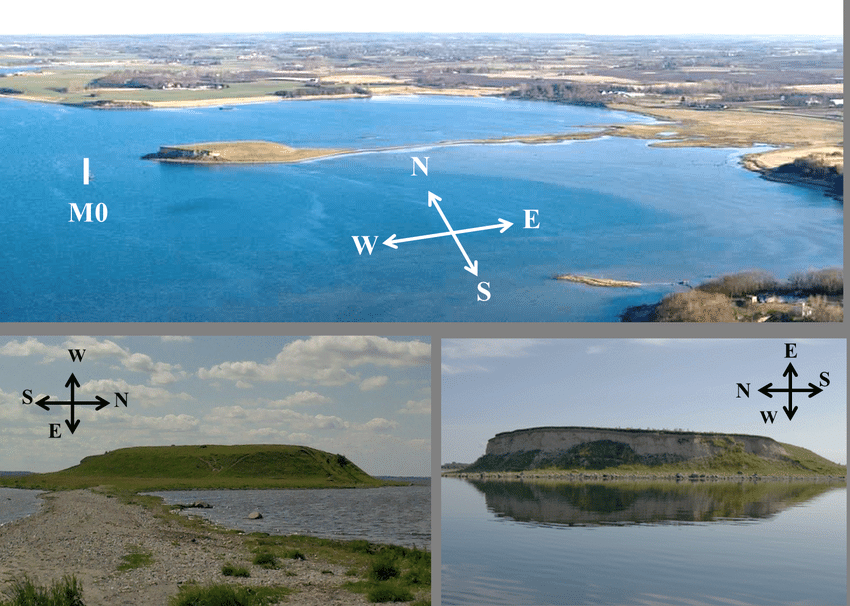
\includegraphics[width=0.98\linewidth,page=1,trim={0cm 0cm 0cm 0cm},clip]{Imagenes/05/bolund}}%
	\caption{Fotografías de la colina de Bolund. Fuente: \cite{phdthesis}}
	\label{fig:05_terreno_bolund}
\end{figure}

\newpage
\section{Preproceso de la Información}
%Las condiciones de borde y de entrada al modelo son las encargadas de definir temporalmente y espacialmente el dominio. Una mala elección de una de ellas puede perjudicar enormemente las soluciones y arruinar toda una simulación, debido a que las ecuaciones a resolver son especialmente sensible a sus condiciones de borde.
\subsection{Condiciones de Borde de Suelo}
La información estática que sirve como condición de borde inferior al modelo debe extraerse de datos satelitales u otros similares con el objetivo que sea uniforme y confiable. Esta información debe ser siempre georeferenciada (protocolo GIS).

WRF utiliza una base de datos estática lo suficientemente amplia como para poder satisfacer un uso normal del modelo. Sin embargo, si se desea utilizar WRF en condiciones extremas, es decir, a escalas lo suficientemente pequeñas como para que las bases de datos no satisfagan la resolución, es necesario actualizar algunas de estas. La información a actualizar será:
\begin{itemize*}
	\item Altura del Terreno: Para una obtención precisa de los niveles $\eta$ en cada punto del dominio y por lo tanto una correcta representación del terreno complejo que es el principal generador de la turbulencia.
	\item Uso de Suelo: Posee la información acerca del \% de vegetación, coeficiente térmico superficial y, lo más importante, el coeficiente de rugosidad ($z_0$), que es el parámetro necesario para estimar los flujos superficiales y la velocidad de fricción.
\end{itemize*}
Las bases de datos a utilizar en las simulaciones son:
\begin{itemize*}
	\item GMTED2010: Dataset por defecto del WRF para la altura del terreno. Obtenida el año 2010 por la USGS y la NGA con una resolución de 30'.
	\item ASTER: Es el único instrumento de alta resolución de la NASA ubicado en la plataforma Terra. Esta base de datos se hizo pública el año 2011 y entrega información de la altura del terreno con una resolución de 1' ($\approx 30$ [m]). Esta es la base de datos que utiliza Google.
	\item USGS: Dataset de uso de suelo que viene por defecto con el WRF. Está basado en mediciones hechas por el satélite AVHRR entre Abril de 1992 y Marzo de 1993 a una resolución de aproximadamente 1 [km].
	\item MODIS: Información sobre uso de suelo obtenida por lo satélites de la NASA. Entrega información en 20 categorías a una resolución de 15'.
	\item Corine: Información de uso de suelo obtenida el año 2012 (proyecto CLC12) a través de imágenes satelitales con 100m de resolución para toda Europa. Posee 44 categorías y es la base de datos de uso de suelo abierta de más alta resolución existente hasta ahora. Para este trabajo se usa la versión 18.5 modificada del año 2016.
	\item Bolund: Los autores del experimento de Bolund entregan bases de datos para la orografía y el coeficiente de rugosidad con una resolución de 25 [cm].
\end{itemize*}
\subsubsection{Incorporación a WRF}
Ls datos descritos anteriormente, muchas veces no están en el formato con el que el preprocesador del modelo WRF (WPS) puede asimilarlo. Sin embargo, debido a los estándares exigidos para información georeferenciada, es posible manipularla de tal manera que puedan incorporarse al modelo. A continuación se describen algunos trabajos que debieron hacerse con las bases de datos.
\begin{itemize*}
	\item ASTER: Cambio de formato de GeoTiff a binario.
	\item Bolund Oro.: La información entregada por el experimento Bolund está dada en un datum UTM Z32, por lo cuál se debe transformar a datum WSG84. Además, debido a la lectura de la información, los autores trasladaron las coordenadas, por lo cual hubo que invertir esta traslación. Se debió transformar la altura del agua entregada (los autores por motivos de interpolación de mareas declaran un $z=0.75$ para agua) a un nivel de $z=0$, para un correcto uso del modelo. 
	\item Corine: Se debió transformar su datum nativo de ETRS89 a WSG84 debido a que la clasificación de suelo por Corine no está implementada en WRF. Se debe hacer un remapeo de los índices al formato USGS. Este procedimiento está descrito por \cite{Pineda2004}. Por otra parte, la resolución de los datos CLC12 son bastante gruesos en comparación con los entregados por ASTER. Luego el WPS presentó algunos errores en reconocer las masas de tierra y para solucionar esto se procedió a hacer una afinación manual de los datos CLC12 en las zonas relevantes para la simulación. Esta afinación puede verse en el Apéndice 2.
	\item Bolund LU: Los autores del experimento entregan información acerca del $z_0$ en el dominio de Bolund y en el mismo formato en el que entregan la orografía, por lo que se debieron hacer las mismas trasformaciones detalladas anteriormente y luego hacer calzar la información entregada con un índice de tipo de suelo y que además fuera consistente con las bases de datos de uso de suelo usadas en los dominios mas grandes.
\end{itemize*}
\subsection{Condiciones de Borde Laterales}
Las simulaciones realizadas contemplan la utilización de una reducción dinámica de escalas (\emph{dynamic downscaling}) a través de dominios anidados, por lo cual se reconocen dos tipos de condiciones de borde para los dominios.
\begin{enumerate*}
	\item[a.] \textbf{Condiciones de borde en el dominio padre:} Provienen de los resultados del reanálisis del modelo global GFS con resolución de $0.5^\circ$ ($\approx 55.6$ [km]). Los resultados o outputs del modelo son obtenidos cada 6 horas por lo cual se realiza una interpolación lineal temporal entre estos para actualizar las condiciones en cada paso de tiempo de este dominio. También, de ser necesario, deben interpolarse espacialmente los valores a las celdas correspondiente según sea la resolución de la malla. La especificación de las condiciones en los bordes es complementada con una zona de buffer (transición) de 5 celdas que permiten suavizar la inclusión de estas al dominio.
	\item[b.] \textbf{Condiciones de borde en los dominios hijos:} Se utilizan los valores coincidentes del borde del dominio interior con las celdas del dominio superior, de esta forma no es necesaria una interpolación temporal, si no que los datos son obtenidos de manera inmediata. Según sea la proporción espacial entre los dominios, la información debe interpolarse desde la malla mas grande a la malla pequeña (generalmente se usan razones 1:3 para definir dominios telescópicos). La implementación de estas condiciones también contempla una zona de buffer, para amortiguar la incorporación de la tendencia en el borde, de 5 celdas.
\end{enumerate*}
Por otra parte, como el dominio mas grande a simular cae dentro de lo que es una simulación de mesoescala y tomando en consideración las proyecciones debido a la curvatura de la tierra para esta zona en particular, se decide fijar la condición de borde superior para la coordenada vertical de presión a $p_{dht} = 30000$ [Pa].

La condición de borde inferior queda determinada por la información obtenida en los datos de uso de suelo para cada punto de la malla y la parametrización de capa superficial.
\subsection{Condiciones Iniciales}
Para inicializar el modelo se utilizan los datos de los análisis  provenientes del modelo  GFS con resolución de $0.5^\circ$ interpolados a cada celda de la malla.

Además, se debe considerar que debido al esquema de clausura LES, es necesario dar un tiempo de adaptación (o \emph{spinup}) para que el modelo pueda desarrollar la turbulencia dentro del flujo. Siguiendo la recomendación del manual del WRF y diversos autores, se decide utilizar un intervalo de tiempo de 6 horas desde el inicio del modelo hasta el momento en que se extraen los resultados para cumplir esto.

\newpage
\section{Descripción del Proceso de Asimilación de Datos}
El proceso de asimilación de datos toma las siguientes consideraciones:
\begin{itemize*}
	\item Debido a la frecuencia de los datos experimentales que se tienen (que es de 10 minutos), la asimilación de datos está limitada a esta misma frecuencia o menor. Por lo tanto, para este experimento se decide utilizar una frecuencia de asimilación de datos de 10 minutos.
	\item Solo se considera ejecutar la asimilación de datos en los dominios interiores (malla más fina) en cada uno de los casos, esto debido a la resolución espacial de estos, es decir, que no se justifica una asimilación de datos en dominios mas gruesos ya que afectaría a una zona mas grande de lo que representa la medición real.
	\item La ventana de tiempo en la cuál se llevará a cabo la asimilación será aquella coincidente con el \emph{spinup} del modelo, de modo que, acabadas las primeras 6 horas de simulación con asimilación, automáticamente se comienzan a recopilar los resultados. Esto tiene como consecuencia que se ejecutan un total de 37 procesos de asimilación.
\end{itemize*}
Un esquema del funcionamiento del DA se presenta en la figura \ref{fig:05_da}. Fuente: Elaboración propia.

\begin{figure}[H]
	\centering
		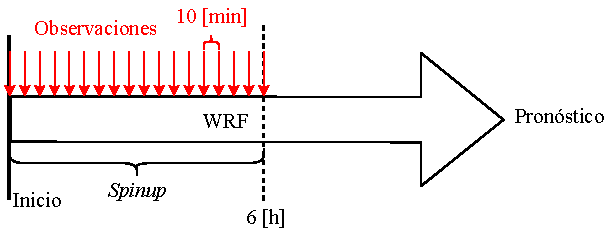
\includegraphics[width=0.95\linewidth,page=1,trim={0cm 0cm 0cm 0cm},clip]{Imagenes/05/da}%
	\caption{Esquema del proceso de asimilación de datos.}
	\label{fig:05_da}
\end{figure}

El modelo WRF se corre durante 10 minutos, luego se extrae el archivo de resultados \emph{.netcdf} y a este se le realiza la asimilación a través de la librería WRFDA. El output de este proceso se reincorpora como condición de borde para el dominio mas interior y luego se vuelve a ejecutar el modelo. Este proceso se sigue realizando iterativamente a través de un script en \emph{bash}.

La recursividad del proceso y el hecho de que la asimilación de datos se lleva a cabo a medida que el modelo integra le da la cualidad de \textbf{Asimilación de Datos 4D}.

Con respecto a la modelación de la matriz $\textbf{B}$, esta es generada a través del método NMC \citep{https://doi.org/10.5065/d68s4mvh} haciendo uso de la herramienta \emph{gen\_be} incluida dentro del mismo código WRFDA. Las constantes de ponderación que usa internamente el WRFDA se fijan con los valores: \emph{var\_scaling} $=1000.0$ y \emph{len\_scaling} $=1.5$.
\newpage
\section{Detalle de Experimentos}
\subsection{Caso I - Terreno Plano: Høvsøre}
Para validar y comparar resultados, se simula un caso real en terreno cuasi-plano con atmósfera neutra. \cite{Pea2013} identifica como Caso 5 a una ventana de tiempo en la cual se satisface esta condición para Høvsøre. Dentro de esta ventana de tiempo, se selecciona un intervalo de 8 horas para que sea aquel en el que la simulación será válida. A estas 8 horas de simulación válida se le deben sumar las 6 horas de simulación precursora (\emph{spinup}) y asimilación de datos, dando un total de 14 horas de simulación.

En la Tabla \ref{tab:05_config_hov} se exponen todos los detalles relevantes a la selección de los dominios numéricos de tal modo que el experimento pueda ser replicado.

\begin{table}[h!]
	\caption{Dominio numérico espacial y temporal para simulación del caso Høvsøre.}\label{tab:05_config_hov}
	\centering\footnotesize
	\begin{tabular}{lcc}
		\toprule
		Parámetro & Selección \\
		\midrule
		Fecha	 	 & 2010-09-08   \\
		Hora Inicio	 	 & 06:00:00   UTC \\
		Hora Término	 		 & 20:00:00 UTC  \\
		Puntos Malla Vert.	 	 & 37   \\
		$P_{top}$ 	& 30000 [Pa]\\
		\# Dominios	& 7   \\
		Lat. Centro	& 56.440588   \\
		Lon. Centro	& 8.150896   \\
		Interválo Salida & 10 [min]\\
		Punto de Malla Total & 2831472\\
		\bottomrule
	\end{tabular}
\end{table}

La selección de los distintos dominios anidados se realizó tomando en consideración la resolución de las condiciones de borde el modelo GFS y las problemáticas que introduce la zona gris de la turbulencia a medida que la malla se va afinando. Para la correcta implementación de las condiciones de borde, se decidió utilizar un criterio conservador y usar una malla inicial (d01) con una resolución aproximada a la del modelo GFS. Luego, los dominios telescópicos irán reduciendo su malla en una razón de 3:1 tal como se recomienda en aplicaciones de mesoescala. La zona gris es pasada por alto al utilizar un criterio análogo al usado por \cite{Green2015}, que utiliza una razón de 5:1 para los dominios en el límite LES (d04-d05). El resto de los dominios seguirán escalando 3:1 hasta una resolución de malla de 25 [m]. Todos los dominios son ubicados de manera telescópica centrados en el mástil meteorológico de la estación.

En la Figura \ref{fig:05_dom_hov} se puede ver la manera en la que se distribuyen los 7 dominios para este caso, además se muestra el detalle de la estructura vertical de la malla para la zona cercana al suelo.

\begin{figure}[H]
	\centering
	\begin{minipage}{0.5\linewidth}
		\center(a)
	\end{minipage}%
	\begin{minipage}{0.5\linewidth}
		\center(b)
	\end{minipage}%
	
	\includegraphics[width=0.45\linewidth,trim={0cm 0cm -0cm 0cm},clip,frame]{Imagenes/05/hov_dom1_edit.jpg}\hspace{0.5cm}%
	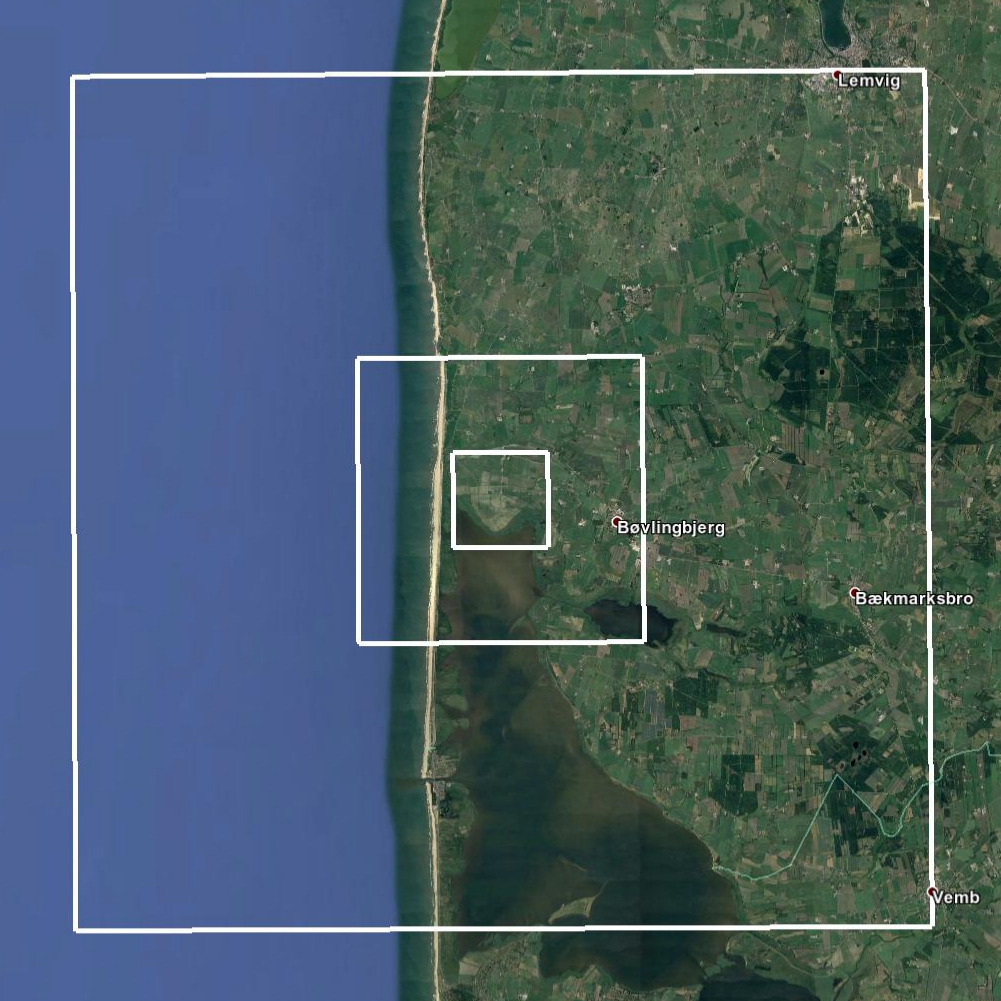
\includegraphics[width=0.45\linewidth,trim={0cm 0cm 0cm 0cm},clip,frame]{Imagenes/05/hov_dom2_edit.jpg}\vspace{0.3cm}%
	
	\begin{minipage}{0.5\linewidth}
		\center \hspace{1.5cm}(c)
	\end{minipage}%
	\begin{minipage}{0.5\linewidth}
		\center(d)
	\end{minipage}%
	
	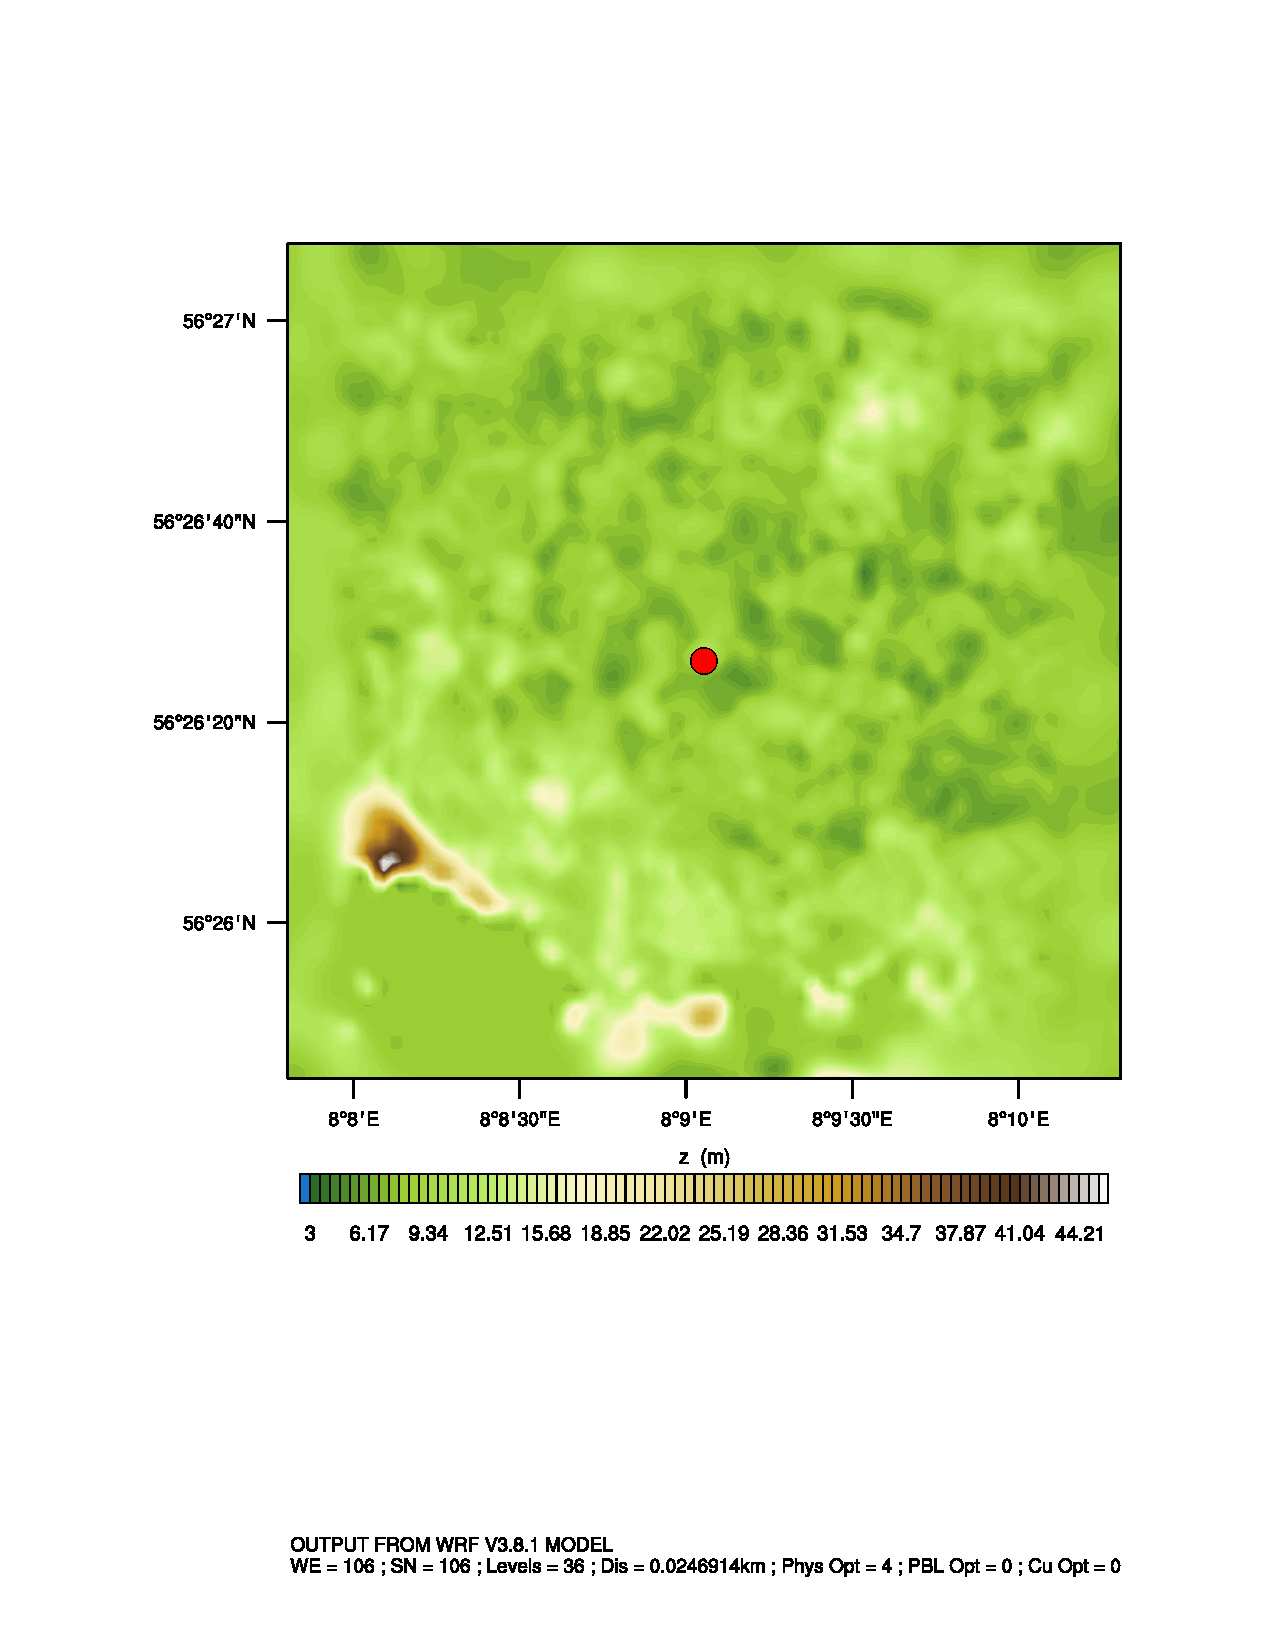
\includegraphics[width=0.45\linewidth,trim={2.5cm 6.5cm 2cm 3.5cm},clip]{Imagenes/05/hov_control_point.pdf}%
	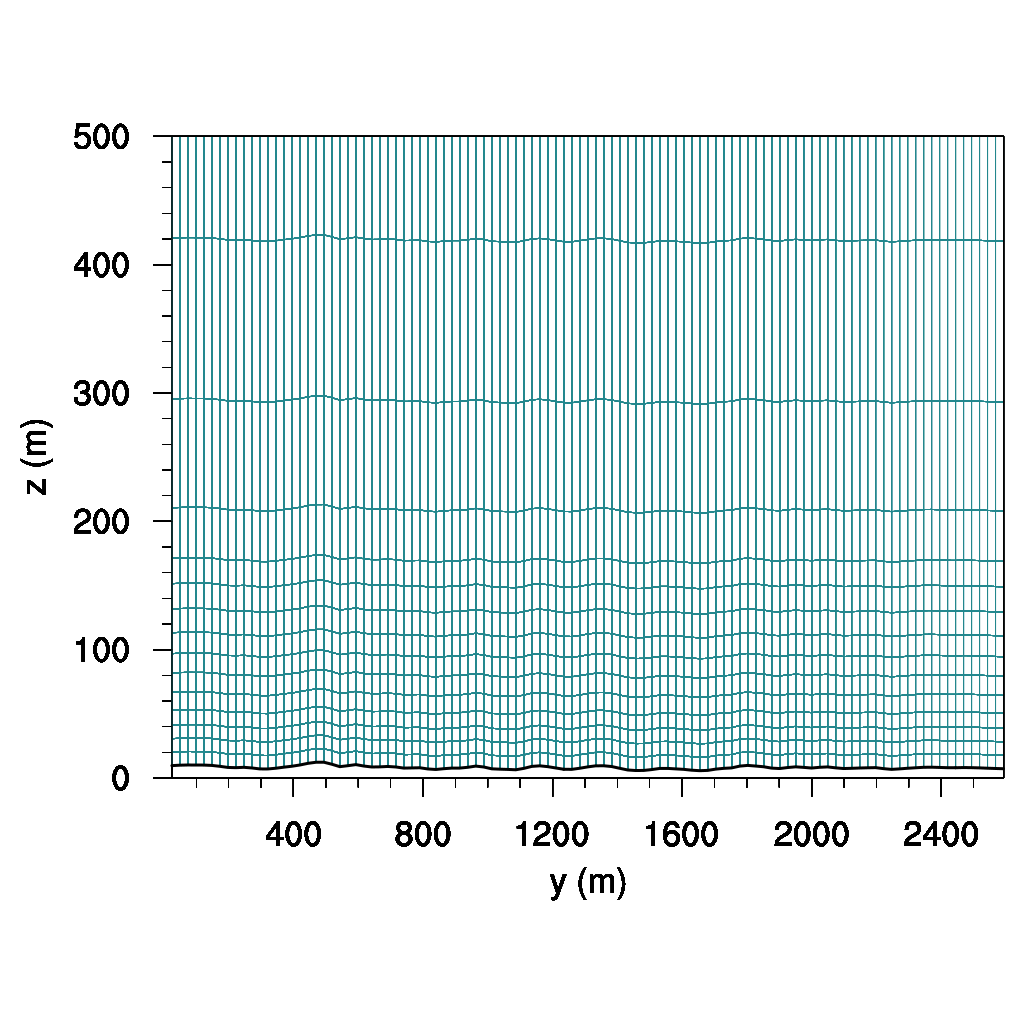
\includegraphics[width=0.45\linewidth,trim={0.5cm 0cm 0cm -1.3cm},clip]{Imagenes/05/mesh57}%
	
	\caption{Información de los dominios de simulación para el caso Høvsøre. (a) Dominios d01-d04. (b) Dominios d05-d07. (c) Dominio d07 con el punto de control. (d) Distribución vertical de la malla adaptativa en escala 4:1.}
	\label{fig:05_dom_hov}
\end{figure}

Las mallas numéricas tienen $107\times107$ nodos en la dirección horizontal y 37 nodos en la dirección vertical. La malla vertical incluye un afinamiento en la cercanía del suelo hecho de tal manera que existan por lo menos 10 puntos en los primeros 100 metros de altura. 

Para el intervalo temporal se aplica el criterio recomendado por los desarrolladores $\Delta t \sim 3\Delta x$, donde $\Delta x$ se prescribe en [km]. De este modo se fija el $\Delta t$ para la primera malla en 90 [seg], sin embargo debido a que el modelo debe tener outputs cada 10 minutos de manera exacta, se decide bajar el paso de tiempo a 75 [seg] (para la malla mas gruesa).

Con respecto a los esquemas de parametrización para las fenomenologías físicas y la utilización de distintas bases de datos, la selección de estos esta detallada en las Tablas \ref{tab:05_caract_hov} y \ref{tab:05_param_hov}. Para el dominio mas interior (d07), se modifica la categoría de uso de suelo de modo que el valor del largo de rugosidad $z_0$ sea el mismo que se entrega en la literatura de \cite{Pea2013}. Para este caso se utiliza un $z_0 = 1.5$ [cm].

\begin{table}[h!]
	\caption{Valores característicos de cada dominio en Høvsøre.}\label{tab:05_caract_hov}
	\centering\footnotesize\resizebox{\textwidth}{!}{
	\begin{tabular}{lccccccc}
		\toprule
		Dominio 				& d01	&	d02	&	d03	&	d04	&	d05	&	d06 &	d07 \\
		\midrule
		$N_x$		& 107 & 107 & 107 &107&107&107&107  \\
		$N_y$	 		& 107 & 107 & 107 &107&107&107&107  \\
		$\Delta x, y$	[m]	 		& 30000 & 10000 & 3333.3 &1111.1&222.22&74.074&24.691  \\
		$\Delta t$	[s]	 		& 75 & 25 & 8.333 &2.778&0.556&0.185&0.062  \\
		Orografía		 	& GMTED & GMTED & GMTED &ASTER&ASTER&ASTER&ASTER  \\
		Uso de Suelo					& USGS & USGS & USGS &CLC12&CLC12&CLC12&CLC12 \\
		\bottomrule
	\end{tabular}}
\end{table}

\begin{table}[h!]
	\caption{Parametrizaciones físicas utilizadas en el modelo para Høvsøre.}\label{tab:05_param_hov}
	\centering\footnotesize\resizebox{\textwidth}{!}{
	\begin{tabular}{lccccccc}
		\toprule
		Dominio 				& d01	&	d02	&	d03	&	d04	&	d05	&	d06 &	d07 \\
		\midrule
		Micro-físicas		 	& WSM5 & WSM5 & WSM5 &WSM5&WSM5&WSM5&WSM5  \\
		Cúmulos			 		& Grell & Grell & -- & -- & -- & -- & -- \\ 
		Capa Superficial	 	& MYNN & MYNN & MYNN & MYNN & MYNN & MYNN & MYNN \\
		PBL				 		& MYNN & MYNN & MYNN & MYNN & -- & -- & -- \\
		Modelo LES				 		& -- & -- & -- & -- & 1.5TKE & 1.5TKE & 1.5TKE \\
		$c_k$				 		& -- & -- & -- & -- & 0.3 & 0.3 & 0.3 \\
		Modelo de Suelo 		& Difus.\footnotemark & Difus. & Difus. & Difus. & Difus. & Difus. & Difus. \\
		Rad. Onda Larga	& RRTM &RRTM&RRTM&RRTM&RRTM&RRTM&RRTM \\
		Rad. Onda Corta	& Dudhia &Dudhia&Dudhia&Dudhia&Dudhia&Dudhia&Dudhia \\
		\bottomrule
	\end{tabular}}
\end{table}

\footnotetext{Modelo de difusión térmica de 5 capas.}

La elección de las parametrizaciones se hizo en base a tres criterios: (i) El uso recomendado por los desarrolladores, (ii) El uso de aquellos que están presentes en las últimas investigaciones relacionadas con WRF y (iii) Un análisis de sensibilidad a cada esquema, el cuál no se muestra en este informe debido a su extensión.

Para el proceso de asimilación de datos se utiliza la información medida en el único mástil meteorológico. Este hecho caracteriza a este experimento como \textbf{Asimilación de Datos de un solo punto o Puntual}. El mástil entrega información cada 10 [min] y en 6 niveles distintos (10, 40, 60, 80, 100 y 116,5 [m])\footnote{Los valores que se asimilan para la velocidad son los mismos que se muestran en la Figura \ref{fig:06_hov_ts}.}. Para el DA solo se asimilan los primeros 5 niveles de estos. Las variables a asimilar en el modelo son las componentes horizontales de la velocidad $u,v$. El detalle de la configuración de la asimilación de datos se muestra en la Tabla \ref{tab:05_config_da_hov}.

\begin{table}[h!]
	\caption{Características del proceso de DA en Høvsøre.}\label{tab:05_config_da_hov}
	\centering\footnotesize
	\begin{tabular}{lcc}
		\toprule
		Parámetro & Selección \\
		\midrule
		Hora Inicio	DA 	 & 06:00:00   \\
		Hora Término DA	 		 & 12:00:00  \\
		Intervalo de DA	&	10 [min] \\
		Puntos a Anidar	 	 & 1   \\
		Alturas 	& 10m, 40m, 60m, 80m, 100m \\
		Variables	& $u,v$   \\
		Lat. Mástil	& 56.440582   \\
		Lon. Mástil	& 8.150896   \\
		
		\bottomrule
	\end{tabular}
\end{table}
\newpage
Los resultados a mostrar para este caso incluirán lo siguiente:
\begin{enumerate*}
	\item [a.]Estimación de la altura o espesar de capa límite.
	\item [b.]Validación del modelo comparando con resultados de \cite{Pea2013}.
	\item [c.]Resultados de primer y segundo orden en el dominio interior.
	\item [d.]Comparación de las series de tiempo medidas y simuladas en el mástil con sus correspondientes momentos estadísticos.
	\item [e.]Mejoras alcanzadas con el proceso de asimilación de datos.
\end{enumerate*}

\newpage










\subsection{Caso II - Terreno Complejo: Bolund}
Tomando en cuenta que la campaña de medición para el caso Bolund se llevó a cabo durante los meses de Diciembre 2007 y Febrero del 2008, fue necesario hallar un día en donde hubiera una estratificación atmosférica lo mas neutra posible, para tener resultados comparables con aquellos obtenidos en la literatura y simulados de manera ideal.

Convenientemente, en el informe técnico que detalla la campaña de medición experimental \citep{3d4285ac04444eb3b9775baf9af052c6}, los autores presentan un gráfico para la longitud de Monin-Obukhov que permite identificar que el día 29 de Diciembre en la tarde se presentan una estratificación muy cercana a la neutra y por lo tanto se decide simular para esas horas.

Debido a la alta resolución de la simulación y el tiempo de cálculo necesario, se decide reducir la ventana de obtención de resultados a 3 horas. De esta manera el tiempo total de simulación será de 9 horas con 6 horas de \emph{spinup}.

Los detalles de la selección de dominios se pueden ver en la Tabla \ref{tab:05_config_bol}.

\begin{table}[h!]
	\caption{Dominio numérico espacial y temporal para simulación del caso Bolund.}\label{tab:05_config_bol}
	\centering\footnotesize
	\begin{tabular}{lcc}
		\toprule
		Parámetro & Selección \\
		\midrule
		Fecha	 	 & 29-12-2007   \\
		Hora Inicio	 	 & 06:00 UTM\\
		Hora Término	 		 & 15:00 UTM\\
		Puntos Malla Vert.	 	 & 41   \\
		$P_{top}$ 	& 30000 [Pa]\\
		\# Dominios	& 8   \\
		Lat. Centro	& 55.703474   \\
		Lon. Centro	& 12.098854   \\
		Interválo Salida & 5 [min]\\
		Punto de Malla Total & 3465000\\
		\bottomrule
	\end{tabular}
\end{table}

Con respecto al anidamiento de los dominios, se utilizaron los mismos criterios que para el caso de Høvsøre. Sin embargo, para alcanzar ahora la alta resolución se utilizan 8 dominios ubicados de manera telescópica centrados en el centro de la colina. La Figura \ref{fig:05_dom_bol} muestra la manera en la que se disponen estos dominios.

En el dominio mas interior (d08), se ubican 8 de los 10 mástiles que se utilizaron para la campaña de medición. Su distribución en el dominio se puede ver en la Figura \ref{fig:05_d08_bol}. Además la Figura \ref{fig:05_d08_bol} muestra la sección en corte a $239^\circ$ para la cual la comparación ciega de modelos numéricos muestra sus resultados.

Con respecto a las mallas, la distribución de estas a lo largo de todos los dominios siguen las mismas recomendaciones que para el caso I. La malla vertical fue refinada debido a la presencia de la pendiente abrupta, de esta manera ahora se consideró la necesidad de por lo menos 3 niveles bajo la altura máxima de la colina para captar la aceleración del flujo y cumplir con las condiciones para un adecuado LES. Este refinamiento se muestra en la Figura \ref{fig:05_mesh_bol}.

\begin{figure}[H]
	\centering
	\includegraphics[width=0.48\linewidth,page=1,trim={5mm 3mm 3mm 3mm},clip,frame]{Imagenes/05/bol_d1-2-3-4edit.jpg}
	\includegraphics[width=0.48\linewidth,page=1,trim={5mm 3mm 3mm 3mm},clip,frame]{Imagenes/05/bol_d4-5-6edit.jpg}
	
	\bigskip
	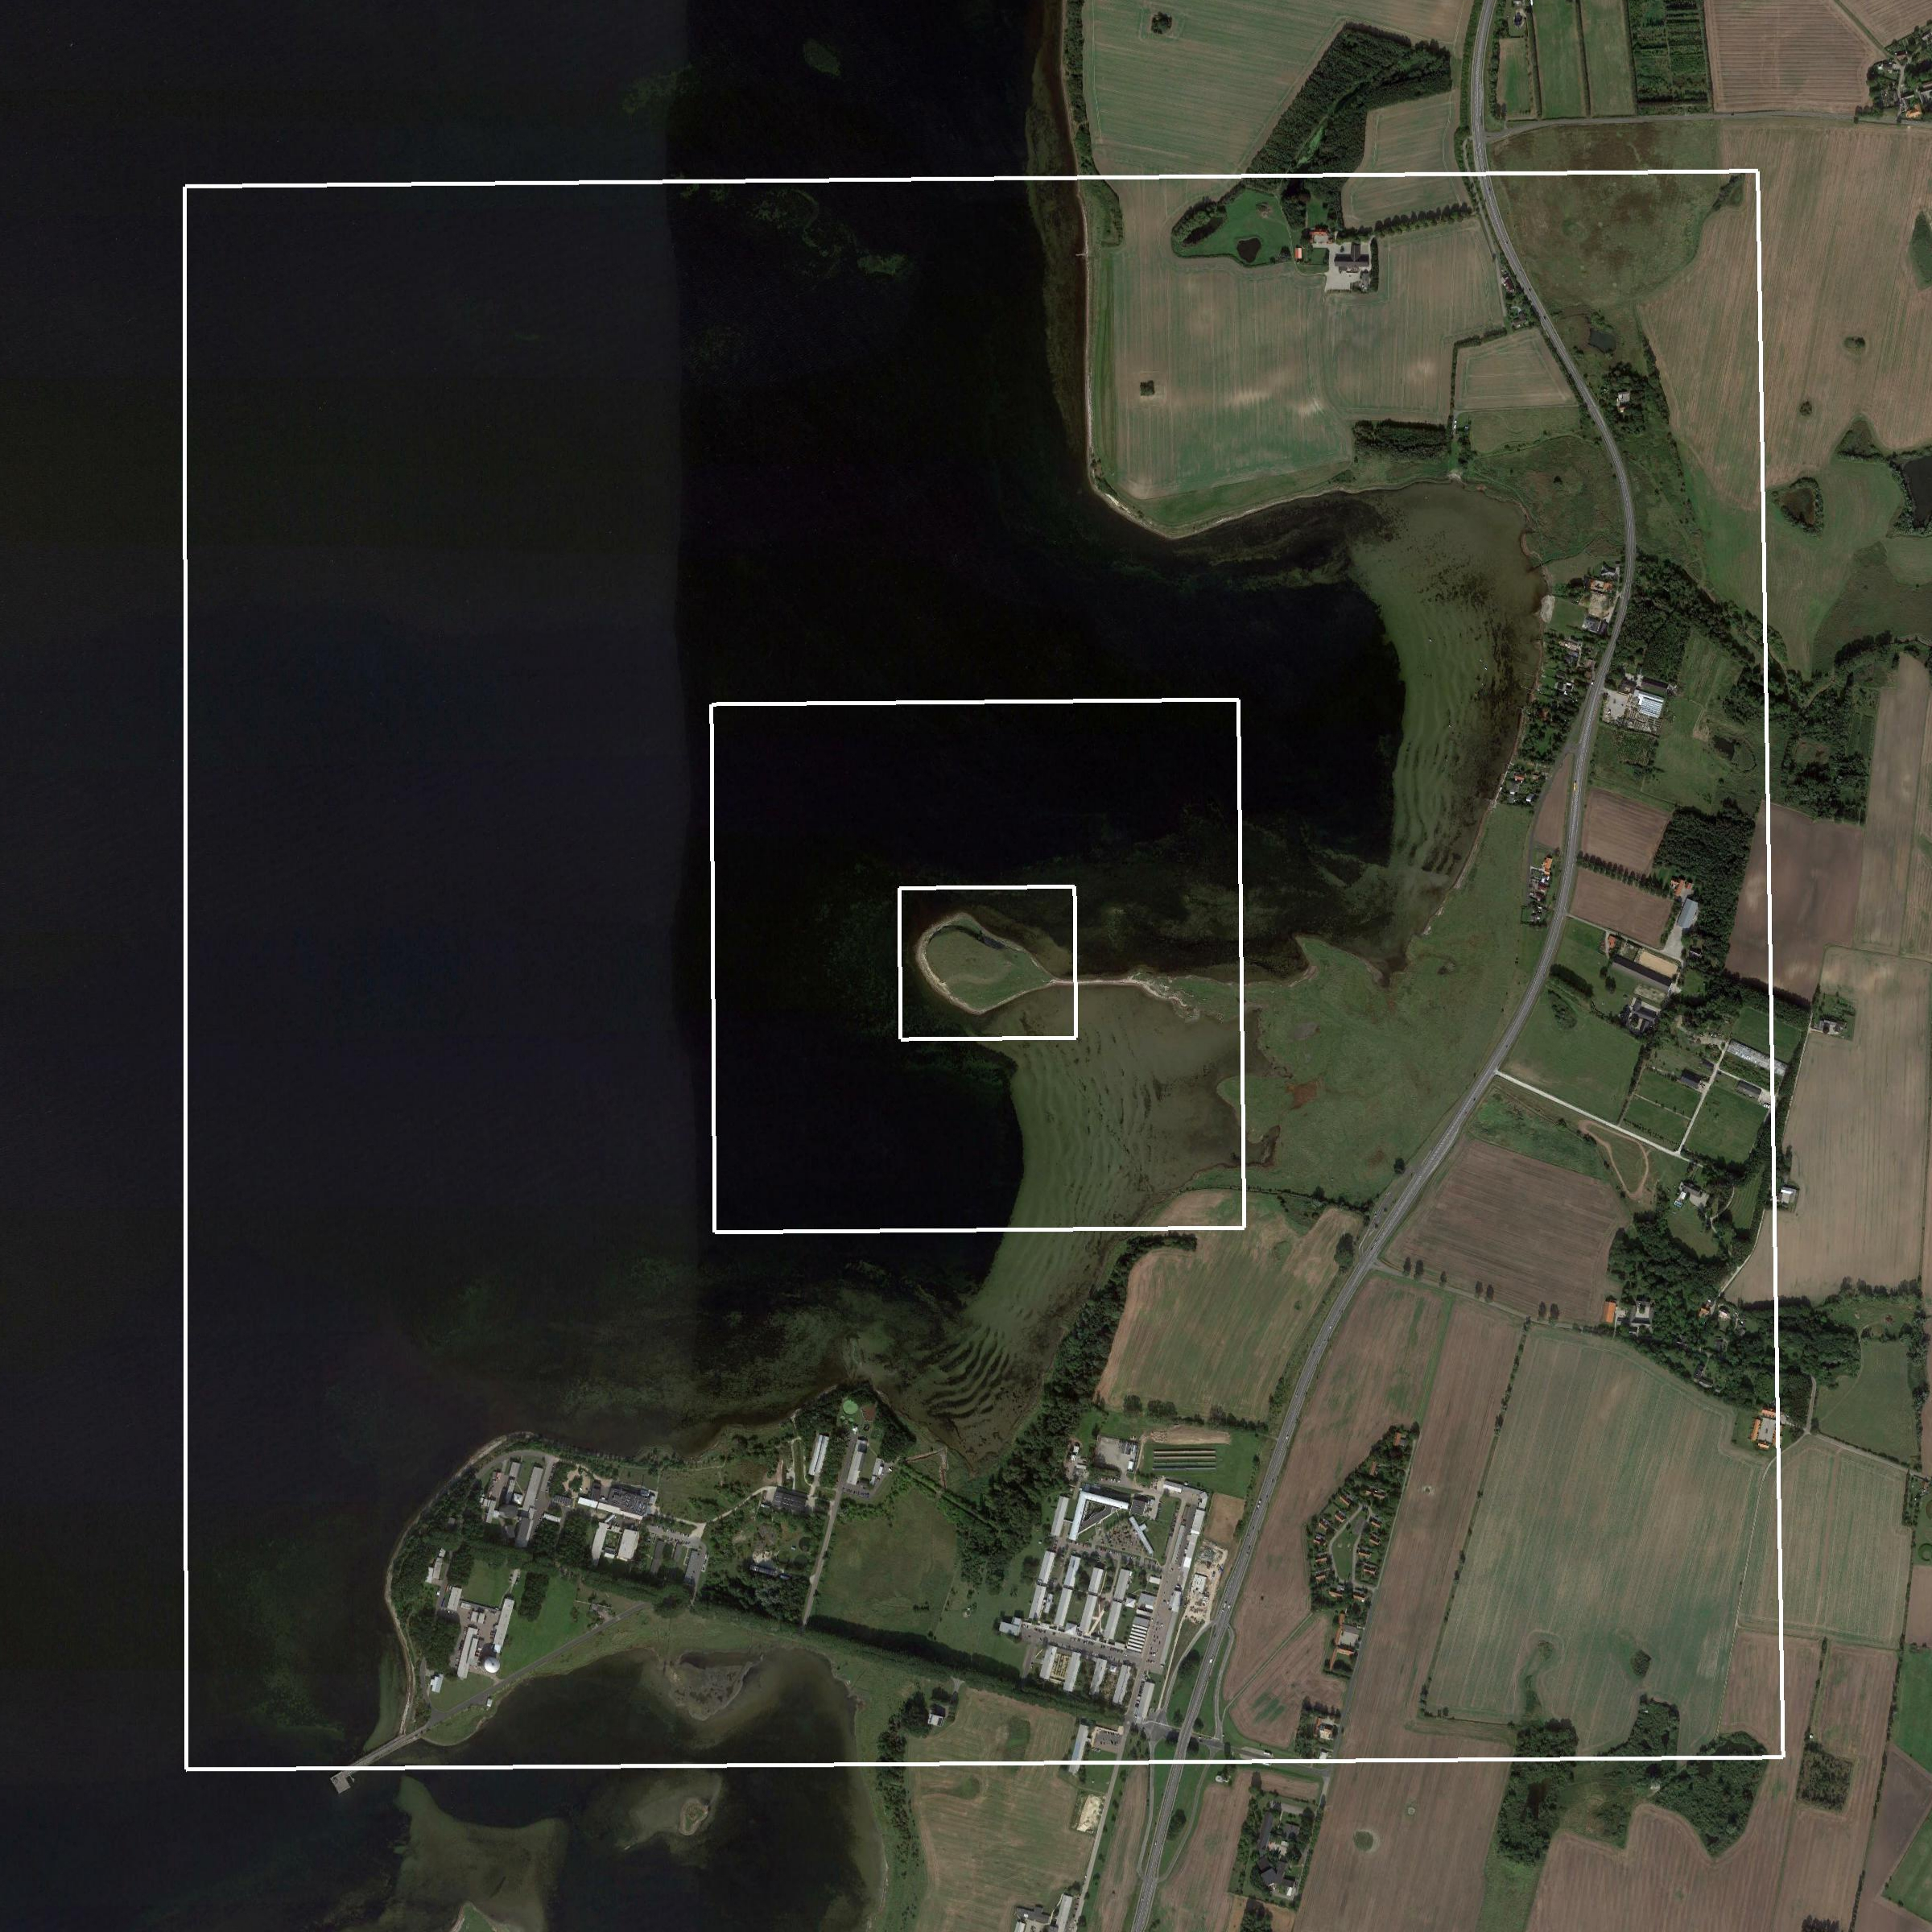
\includegraphics[width=0.48\linewidth,page=1,trim={5mm 3mm 3mm 3mm},clip,frame]{Imagenes/05/bol_d6-7-8edit.jpg}%
	
	\caption{Distribución telescópica de los 8 mallas anidadas en el dominio numérico de la colinda Bolund.}
	\label{fig:05_dom_bol}
\end{figure}

El intervalo temporal también se ve afectado por el terreno complejo provocando que la regla recomendada por los desarrolladores ya no sea válida debido a que en las cercanías de la pendiente abrupta se viola localmente el criterio de estabilidad numérica impuesto por el CFL. Se realizó entonces pruebas de sensibilidad al $\Delta t$ hasta hallar un valor que permitió la estabilidad del modelo durante toda la simulación. Este valor se fijó en $\Delta t = 12$ [s] para el dominio mas grueso (d01).

\newpage
\vspace*{\fill}
\begin{figure}[H]
	\centering
	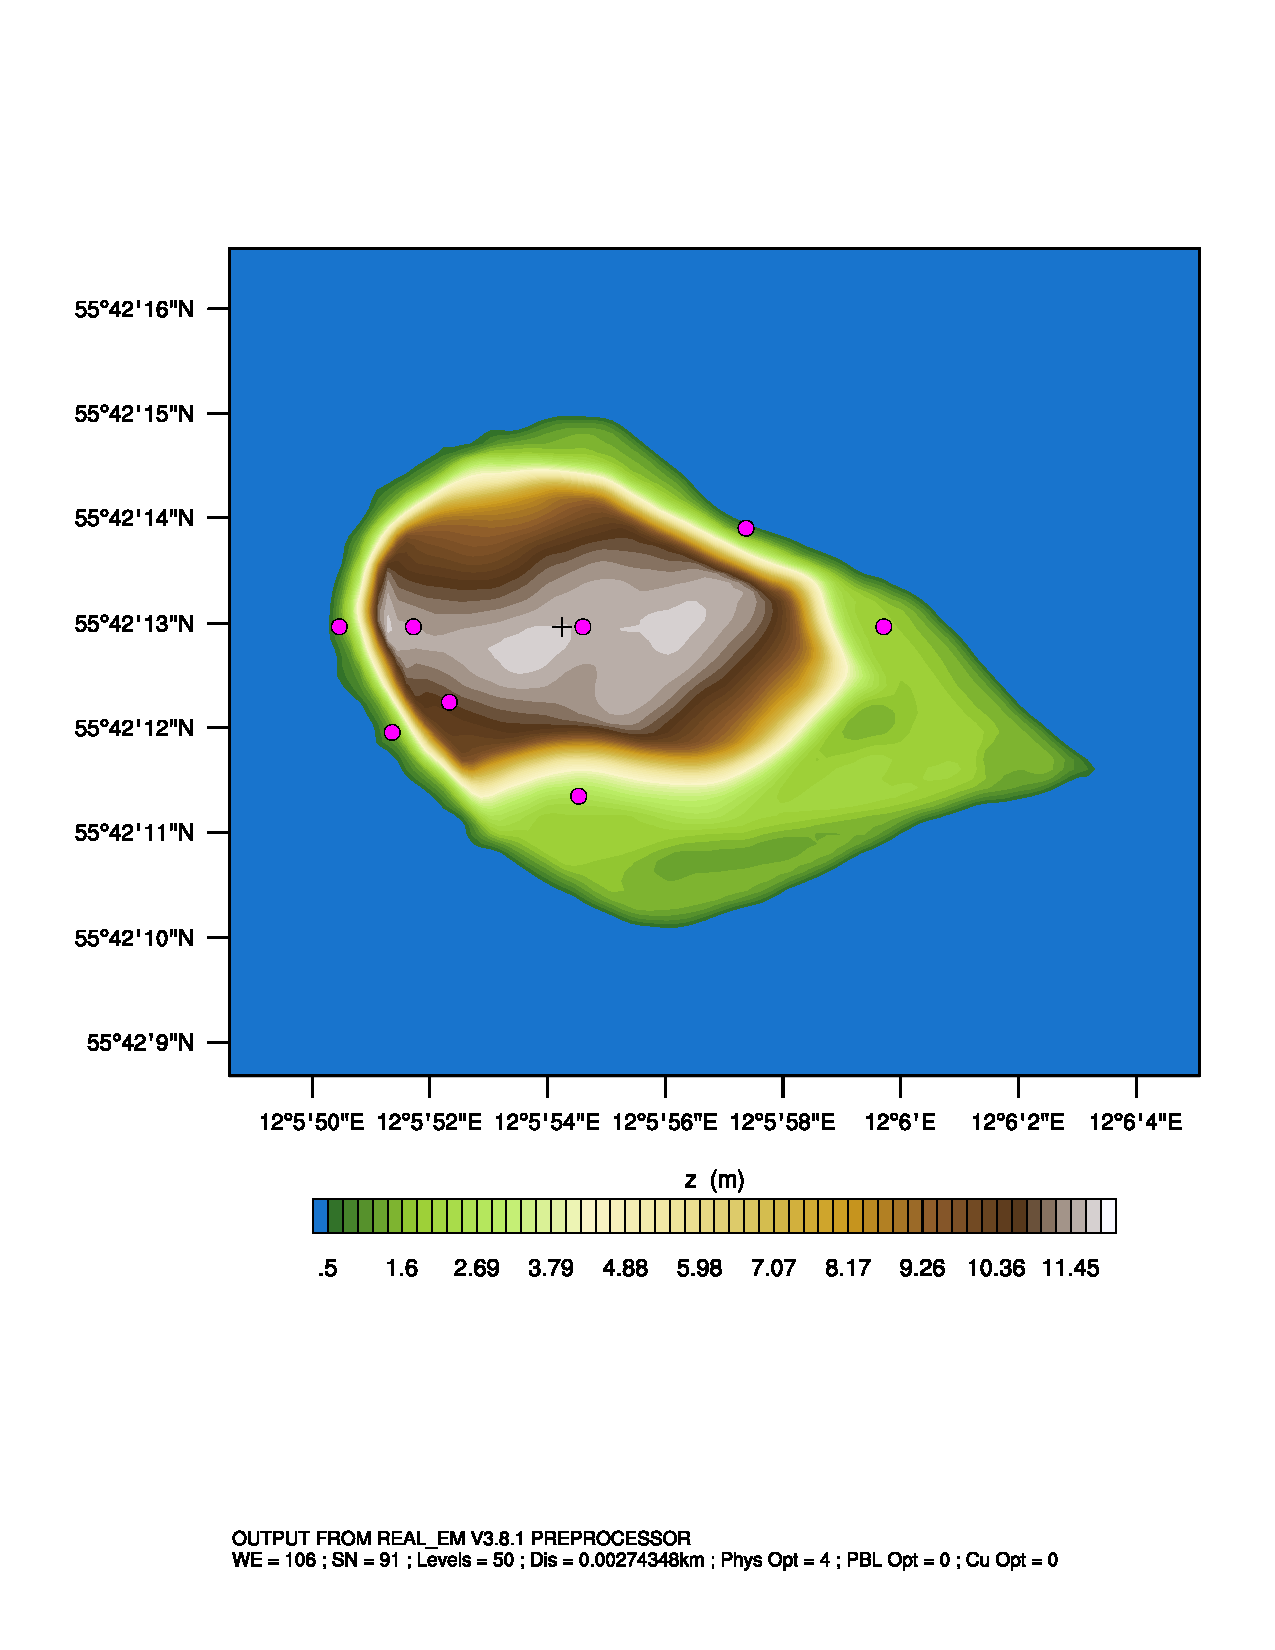
\includegraphics[width=0.9\linewidth,page=1,trim={0cm 6cm -1cm 4cm},clip]{Imagenes/05/bol_control_point.pdf}%
	\caption{Ubicación espacial de los puntos de control en el dominio de Bolund. En cada punto de control se ubican anemómetros que miden a las alturas de 2m, 5m, y 9m sobre el suelo.}
	\label{fig:05_d08_bol}
\end{figure}

\vspace*{\fill}
\begin{figure}[H]
	\centering
	\begin{minipage}{0.5\linewidth}
		\center\hspace{1.8cm}(a)
	\end{minipage}%
	\begin{minipage}{0.5\linewidth}
		\center(b)
	\end{minipage}%
	
	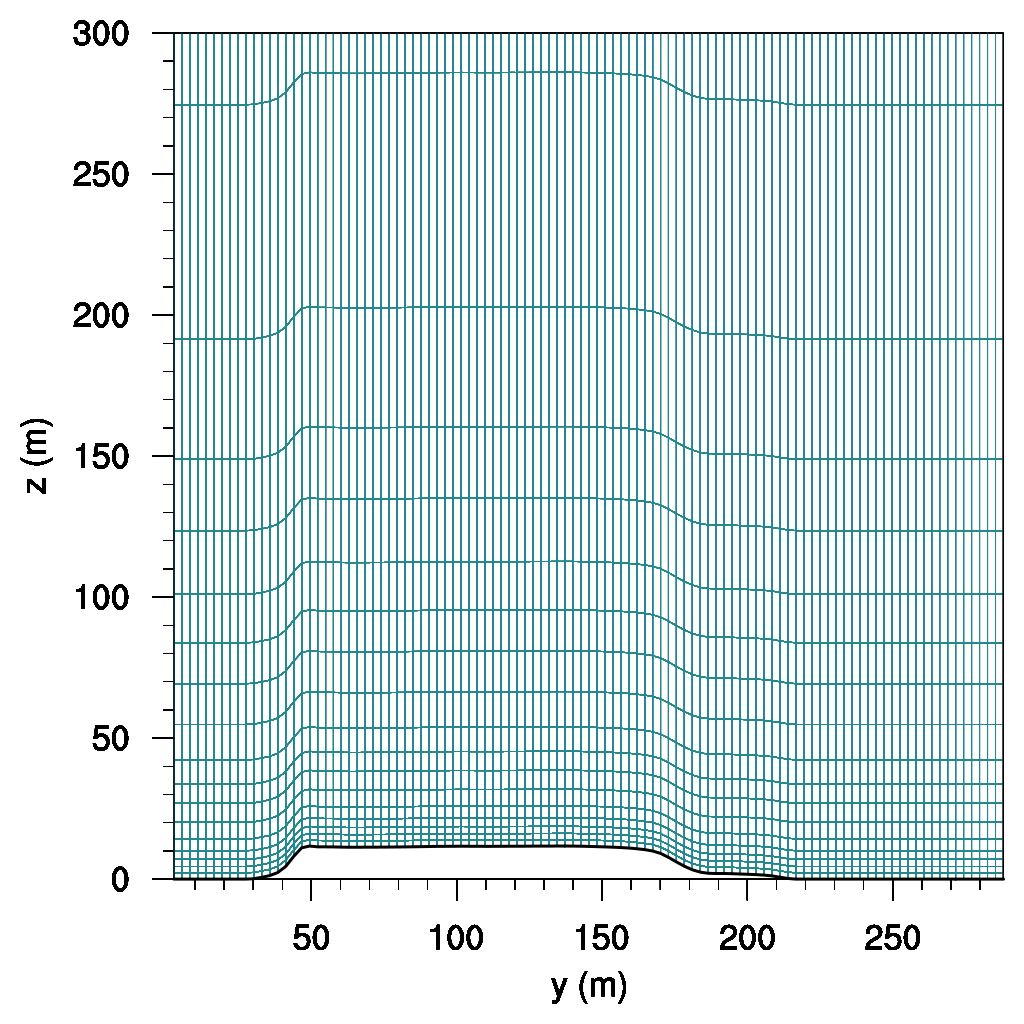
\includegraphics[width=0.45\linewidth,trim={0cm 0cm -0cm 0cm},clip]{Imagenes/05/mesh_y50}%
	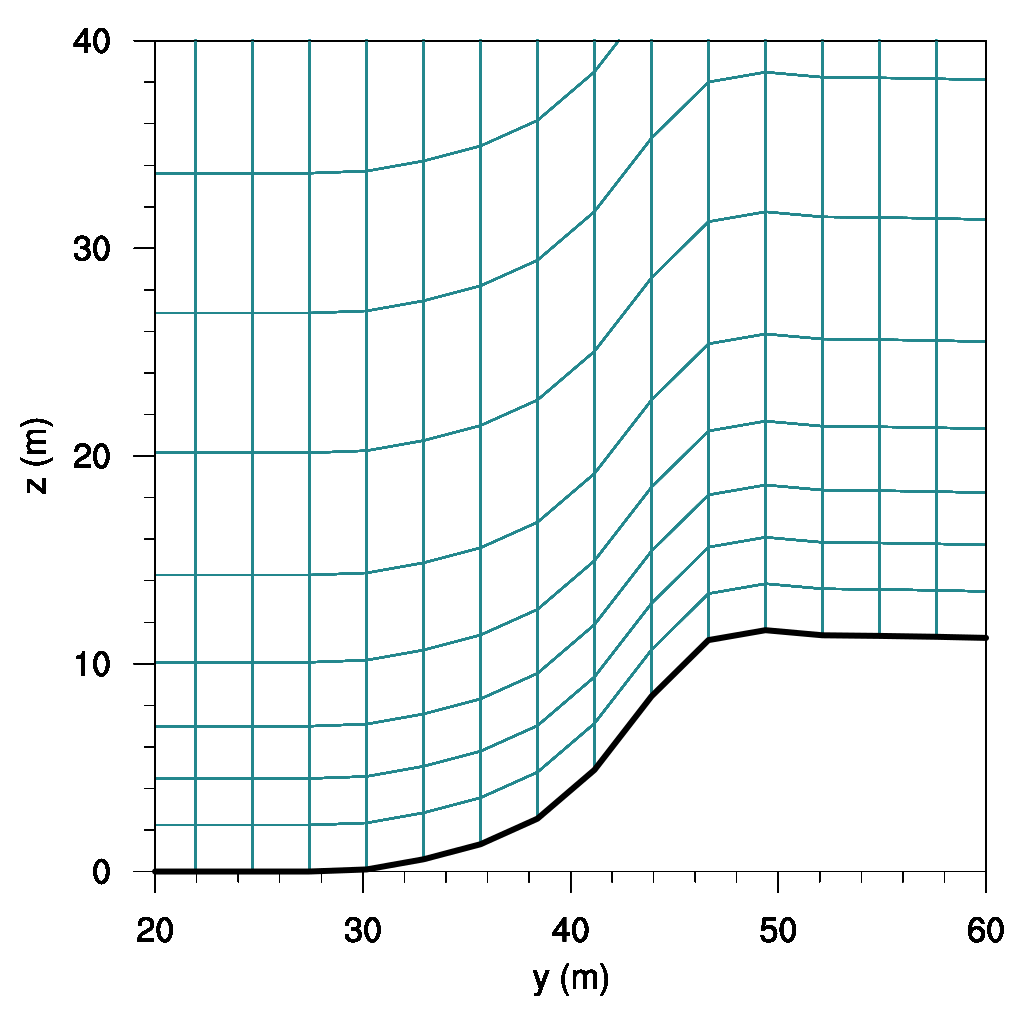
\includegraphics[width=0.45\linewidth,trim={0cm 0cm 0cm 0cm},clip]{Imagenes/05/hd_mesh_50}%
	
	\caption{(a) Distribución de la malla vertical en la mitad del dominio en Bolund. (b) Detalle la pendiente abrupta (escala 1:1).}
	\label{fig:05_mesh_bol}
\end{figure}
\vspace*{\fill}

\newpage
La selección de los esquemas de parametrización se hizo en función de lo resultados obtenidos para el terreno plano. Para las bases de datos de información estática se realiza el mismo procedimiento que para el caso I de Høvsøre, con la distinción de que para el dominio interior (d08) se utilizan las bases de datos entregadas por los desarrolladores del experimento de comparación ciega. El dominio d08 utiliza un largo de rugosidad $z_0=1.5$ [cm] \cite{Bechmann2011}. La información de estos se muestra en las Tablas \ref{tab:05_caract_bol} y \ref{tab:05_param_bol}.

\begin{table}[H]
	\caption{Valores característicos de cada dominio en Bolund.}\label{tab:05_caract_bol}
	\centering\footnotesize\resizebox{\textwidth}{!}{
	\begin{tabular}{lcccccccc}
		\toprule
		Dominio 				& d01	&	d02	&	d03	&	d04	&	d05	&	d06 &	d07&	d08 \\
		\midrule
		$N_x$		& 106 & 106 & 106 &106&106&106&106&106  \\
		$N_y$	 		& 106 & 106 & 106 &106&106&106&106&91  \\
		$\Delta x, y$	[m]	 		& 10000 & 3333.3 & 1111.1 &222.22&74.074&24.691&8.23045&2.74348  \\
		$\Delta t$	[s]	 		& 12 & 4 & 1.3333 &0.4444&0.0889&0.0296&0.0099&0.0033  \\
		Orografía		 	& GMTED & GMTED & GMTED &ASTER&ASTER&ASTER&ASTER&Bolund  \\
		Uso de Suelo		& USGS & USGS & USGS &CLC12&CLC12&CLC12&CLC12&Bolund \\
		\bottomrule
	\end{tabular}}
\end{table}

\begin{table}[H]
	\caption{Parametrizaciones físicas utilizadas en el modelo para Bolund.}\label{tab:05_param_bol}
	\centering\footnotesize\resizebox{\textwidth}{!}{
	\begin{tabular}{lcccccccc}
		\toprule
		Dominio 				& d01	&	d02	&	d03	&	d04	&	d05	&	d06 &	d07& d08\\
		\midrule
		Micro-físicas		 	& WSM5 & WSM5 & WSM5 &WSM5&WSM5&WSM5&WSM5& WSM5 \\
		Cúmulos			 		& Grell & -- & -- & -- & -- & -- & -- & -- \\ 
		Capa Superficial	 	& MYNN & MYNN & MYNN & MYNN & MYNN & MYNN & MYNN& MYNN\\
		PBL				 		& MYNN & MYNN & MYNN & -- & -- & -- & -- &--\\
		Modelo LES				 		& -- & -- & -- & 1.5TKE & 1.5TKE & 1.5TKE & 1.5TKE& 1.5TKE \\
		$c_k$				 		& -- & -- & -- & $0.2$ & $0.2$ & $0.2$ & $0.2$& $0.2$ \\
		Modelo de Suelo 		& Difus. & Difus. & Difus. & Difus. & Difus. & Difus. & Difus.& Difus. \\
		Rad. Onda Larga	& RRTM &RRTM&RRTM&RRTM&RRTM&RRTM&RRTM& RRTM\\
		Rad. Onda Corta	& Dudhia &Dudhia&Dudhia&Dudhia&Dudhia&Dudhia&Dudhia& Dudhia\\
		\bottomrule
	\end{tabular}}
\end{table}

Las asimilación de datos se realiza en los 8 mástiles que se ubican dentro del dominio, y por lo tanto para este experimento se habla de \textbf{Asimilación de Datos Multipunto}. La instrumentación está ubicada aproximadamente a 2, 5 y 9 [m] sobre el nivel del suelo, sin embargo no todos los mástiles poseen los instrumentos necesarios para entregar información sobre la dirección del viento, por lo tanto la asimilación solo se llevará a cabo en aquellos puntos en donde se tiene información sobre la velocidad y la dirección. Los parámetros del proceso de DA se puede ver en las Tablas \ref{tab:05_config_da_bol} y \ref{tab:05_mast_da_bol}. Debe notarse que la asimilación para este caso se hace a niveles muy cercano a la superficie, en comparación al caso de Høvsøre donde se tiene información hasta aproximadamente 100 [m] sobre el nivel del mar.

\begin{table}[h!]
	\caption{Características del proceso de DA en Bolund.}\label{tab:05_config_da_bol}
	\centering\footnotesize
	\begin{tabular}{lcc}
		\toprule
		Parámetro & Selección \\
		\midrule
		Hora Inicio	DA 	 & 06:00:00   \\
		Hora Término DA	 		 & 12:00:00  \\
		Intervalo de DA	&	10 [min] \\
		Puntos a Anidar	 	 & 8   \\
		Variables	& $u,v$   \\
		\bottomrule
	\end{tabular}
\end{table}

\begin{table}[H]
	\caption{Detalle de la asimilación en cada mástil en Bolund.}\label{tab:05_mast_da_bol}
	\centering\footnotesize\resizebox{\textwidth}{!}{
	\begin{tabular}{lcccccccc}
		\toprule
		 				& M1	&	M2	&	M3	&	M4	&	M5	&	M6 &	M7	& M8\\
		\midrule
		Latitud		 	& 55.70332 & 55.70340 & 55.70360 & 55.70386 & 55.70315 & 55.70360 & 55.70360 & 55.70360 \\
		Longitud	    & 12.09760 & 12.09787 & 12.09850 & 12.09927 & 12.09848 & 12.09770 & 12.09735 & 12.09992 \\
		Alturas			& 2, 5, 9m & 2, 5m & 2, 5m & 2, 5, 9m & 2, 5m & 2, 5m & 2, 5m & 2, 5m \\

		\bottomrule
	\end{tabular}}
\end{table}

Finalmente, los resultados relevantes que se mostrarán para este caso son:
\begin{enumerate*}
	\item[a.] Estimación del alto o espesor de la capa límite.
	\item[b.] Resultados de primer y segundo orden en el dominio.
	\item[c.] Comparación con los resultados obtenidos en la comparación ciega para la sección M1-M4.
	\item[d.] Comparación entre las series de tiempo medidas y simuladas, medida del error y correlación.
	\item[e.] Mejoras alcanzadas con el proceso de DA. 
\end{enumerate*}
\newpage
\section{Posproceso de los datos}
\subsection{Interpolación para Series de Tiempo}
Para poder comparar las series de tiempo provenientes de los datos públicos con las series de tiempo simuladas en los puntos de interés, es necesario llevar los datos simulados a las alturas a las cuales se toman las mediciones.

Para esto se utiliza una interpolación en base a la ley de potencia para atmósfera neutra de la forma:
\be 
u(z) = u(z_r)\frac{\ln{(z/z_0)}}{\ln{(z_r/z_0)}}.
\ee
Donde $z_0$ es el alto de rugosidad (que para Høvsøre y Bolund tiene un valor uniforme de $z_0=1.5$ [cm]).
\subsection{Definición de Métricas de Error y Correlación}
Luego de interpolar la simulación a los puntos de interés, es necesario definir una estimación del error entre la simulación realizada y la serie de tiempo medida en el mástil.

Se decide utilizar tres indicadores para llevar a cabo esta tarea: el MAE, el RMSE y el coeficiente de correlación de Pearson.

El MAE (\emph{Mean Absolute Error}) entre dos variables continuas se calcula de la siguiente forma:

\be 
MAE = \frac{1}{n}\sum_{i=1}^n |y_i-x_i|.
\ee

Es un promedio del valor absoluto de los errores. Si se grafica la correspondencia de los datos en un gráfico de $x$ vs $y$, el MAE correspondería al valor medio de la distancia horizontal entre cada punto y la línea $x=y$.

El RMSE (\emph{Root Mean Squared Error}) por otro lado se calcula como:

\be 
RMSE = \sqrt{\frac{1}{n}\sum_{i=1}^n (y_i-x_i)^2},
\ee

que corresponde a la raíz de los momentos muestrales de segundo orden de la diferencia entre los valores a comparar, en otras palabras, es un análogo al MAE pero pondera con mayor importancia los errores mas grandes. Es un promedio de los errores al cuadrado.

Finalmente el coeficiente de correlación de Pearson $r$ corresponde a la razón entre las covarianzas de las dos variables con el producto de sus desviaciones estándar:
\be 
r = \frac{Cov(x,y)}{s_x s_y} = \frac{\sum\limits_{i=1}^n [(x_i-\overline{x})(y_i-\overline{y})]} {\left[\sum\limits_{i=1}^n (x_i-\overline{x})^2\right]^{1/2} \left[\sum\limits_{i=1}^n (y_i-\overline{y})^2\right]^{1/2}}.
\ee

Es un indicador de la proporcionalidad entre los datos simulados y medidos. Idealmente, para este caso, el valor debería ser unitario, lo cual significaría que un valor medido corresponde a un mismo valor simulado.